\newpage 
\onecolumn
\section{Proofs of Theorems}
\label{sec:dsproofs}
Here, we present proofs for theorem and proposition. %To avoid cluttering, during our proofs, we state some needed results as lemmas and provide their proof in the next Section \ref{sec:lemmas}. 
\subsection{Proof of Proposition \ref{prop:super}}
\begin{proof}
	Consider only one group for regression in isolation. 
	Note that $\y_g = \X_g (\bbeta _g^* + \bbeta _0^*) + \oomega_g$ is a superposition model and as shown in \cite{guba16} the sample complexity required for the RE condition and subsequently recovering $\bbeta _0^*$ and $\bbeta _g^*$ is $n_g  \geq c(\max(\omega(\cA_0), \omega(\cA_g) ) + \sqrt{\log 2})^2$.
\end{proof} 
%\subsection{Proof of Theorem \ref{theo:iter}}

%\begin{lemma}
%	\label{lemm:simp}
%	For two random variables $X$ and $Y$ and positive constants $a$ and $b$ we have the followings:
%	\be
%	\nr 
%	\pr \left(XY \leq ab \right) &\leq&  \pr(X \leq a) + \pr(Y \leq b)
%	\\ \nr 
%	\pr \left(X+Y \leq a+b \right) &\leq&  \pr(X \leq a) + \pr(Y \leq b)
%	\ee 
%	Note that $X$ and $Y$ can be dependent, e.g., function of another random variable $Z$.
%\end{lemma}


%Using the result of Lemma \ref{lem:gennips}, in the following Lemma \ref{lem:dec}, we show that the assumption of the Lemma \ref{lem:angel} holds for the two $n$-dimensional vectors $\a = \oomega \ddelta_0$ and  $\b = \D \ddelta_{1:G}$ with high probability  and specifically characterizes the $\epsilon$. 





%%%%%%%%%%%%%% Non-convex trial Begins %%%%%%%%%%%%%%%%%%
%\subsection{Proof of Lemma \ref{lem:recurse}}
%\begin{proof}
%	We upper bound the individual error $\norm{\ddelta_g^{(t+1)}}{2}$ and the common one $\norm{\ddelta_0^{(t+1)}}{2}$ in the followings:
%	\be
%	\nr 
%	\norm{\ddelta_g^{(t+1)}}{2} &=& \norm{\bbeta _g^{(t+1)} - \bbeta _g^*}{2} \\ \nr  
%	&=& \normlr{\Pi_{\Omega_{f_g}} \bigg(\bbeta_g^{(t)} + \mu_g \X_g^T \Big(\y_g - \X_g \big(\bbeta_0^{(t)} + \bbeta_g^{(t)}\big) \Big) \bigg) - \bbeta _g^*}{2} \\ \nr 
%	\text{(Lemma 6.3 of \cite{oyrs15})}&=& \normlr{\Pi_{\Omega_{f_g}-\{ \bbeta _g^* \}} \bigg(\bbeta_g^{(t)} + \mu_g \X_g^T \Big(\y_g - \X_g \big(\bbeta_0^{(t)} + \bbeta_g^{(t)}\big) \Big) - \bbeta _g^* \bigg)}{2} \\ \nr 
%	&=& \normlr{\Pi_{\cE_g} \bigg(\ddelta_g^{(t)} + \mu_g \X_g^T \Big(\y_g - \X_g \big(\bbeta_0^{(t)} + \bbeta_g^{(t)}\big) - \X_g \big(\bbeta _0^* + \bbeta _g^* \big) + \X_g \big(\bbeta _0^* + \bbeta _g^*\big) \Big) \bigg)}{2} \\ \nr 
%	&=& \normlr{\Pi_{\cE_g} \bigg(\ddelta_g^{(t)} + \mu_g \X_g^T \Big(\oomega_g - \X_g \big(\ddelta_0^{(t)}  + \ddelta_g^{(t)}\big) \Big) \bigg)}{2} \\ \nr 
%	\text{(Lemma 6.4 of \cite{oyrs15})}&\leq& \theta_f \normlr{\Pi_{\cC_g} \bigg(\ddelta_g^{(t)} + \mu_g \X_g^T \Big(\oomega_g - \X_g \big(\ddelta_0^{(t)}  + \ddelta_g^{(t)}\big) \Big) \bigg)}{2} \\ \nr 
%	\text{(Lemma 6.2 of \cite{oyrs15})}&\leq& \theta_f \sup_{\v \in \cC_g \cap \ball} \v^T \bigg(\ddelta_g^{(t)} + \mu_g \X_g^T \Big(\oomega_g - \X_g \big(\ddelta_0^{(t)}  + \ddelta_g^{(t)}\big) \Big) \bigg) \\ \nr
%	(\cB_g =  \cC_g \cap \ball) &=& \theta_f \sup_{\v \in \cB_g} \v^T \bigg(\ddelta_g^{(t)} + \mu_g \X_g^T \Big(\oomega_g - \X_g \big(\ddelta_0^{(t)}  + \ddelta_g^{(t)}\big) \Big) \bigg) \\ \nr
%	&\leq& \theta_f \sup_{\v \in \cB_g} \v^T \big(\I_g - \mu_g \X_g^T \X_g\big) \ddelta_g^{(t)} + \theta_f \mu_g \sup_{\v \in \cB_g} \v^T \X_g^T \oomega_g  + \theta_f \mu_g \sup_{\v \in \cB_g} -\v^T \X_g^T \X_g \ddelta_0^{(t)}   \\ \nr
%	&\leq& \theta_f \normlr{\ddelta_g^{(t)}}{2} \sup_{\u, \v \in \cB_g} \v^T \big(\I_g - \mu_g \X_g^T \X_g\big) \u  + \theta_f \mu_g \norm{\oomega_g}{2} \sup_{\v \in \cB_g} \v^T \X_g^T \frac{\oomega_g}{\norm{\oomega_g}{2}}  \\ \nr 
%	&+& \theta_f \mu_g  \norm{\ddelta_0^{(t)} }{2}  \sup_{\v \in \cB_g, \u \in \cB_0} -\v^T \X_g^T \X_g \u \\ \nr   
%	&=& \theta_f \rho_g(\mu_g)\norm{\ddelta_g^{(t)}}{2}   +  \theta_f \xi_g(\mu_g) \norm{\oomega_g}{2} + \theta_f \phi_g(\mu_g) \norm{\ddelta_0^{(t)}}{2} 
%	\ee 
%	where $\theta_f = 1$ for convex $f$ and $\theta_f = 2$ for the non-convex case. 
%%	Note that the last term is lower bounded by zero. To see this clearly consider the set $\cB_{0g} = \{\ddelta_0 + \ddelta_{g} | \ddelta_0 \in \cC_0, \ddelta_g \in \cC_g, \norm{\ddelta_0 + \ddelta_g}{2} \leq 1\}$ where $\cB_0, \cB_g \subseteq \cB_{0g}$:
%%	\be 
%%	\label{eq:zerolb}
%%	\inf_{\v \in \cB_g, \u \in \cB_0} \v^T \X_g^T \X_g \u &\geq& \inf_{\u \in \cB_{0g}} \norm{\X_g \u}{2}^2 \geq 0
%%	\ee 
%	So the final bound becomes:
%	\be 
%	\label{eq:optg}
%	\norm{\ddelta_g^{(t+1)}}{2} &\leq&  \theta_f \left(\rho_g(\mu_g)\norm{\ddelta_g^{(t)}}{2}   +  \xi_g(\mu_g) \norm{\oomega_g}{2} + \phi_g(\mu_g) \norm{\ddelta_0^{(t)}}{2} \right)
%	\ee 	
%	Now we upper bound the error of common parameter. Remember common parameter's update:
%	$\bbeta _0^{(t+1)} = \Pi_{\Omega_{f_0}} \left(\bbeta_0^{(t)} + \mu_0 \X_0^T   
%	\begin{pmatrix}
%	(\y_1 - \X_1 (\bbeta_0^{(t)} + \bbeta _1^{(t)}))     \\
%	\vdots 	 \\
%	(\y_G - \X_G (\bbeta_0^{(t)} + \bbeta _G^{(t)})) 
%	\end{pmatrix}\right)$.
%	\be 
%	\nr 
%	\norm{\ddelta_0^{(t+1)}}{2} &=& \norm{\bbeta _0^{(t+1)} - \bbeta _0^*}{2} \\ \nr  \\ \nr 
%	&=& \normlr{\Pi_{\Omega_{f_0}} \bigg(\bbeta_0^{(t)} + \mu_0 \sum_{g = 1}^{G} \X_g^T \Big(\y_g - \X_g (\bbeta_0^{(t)} + \bbeta_g^{(t)}) \Big) \bigg) - \bbeta _0^*}{2} \\ \nr 
%	\text{(Lemma 6.3 of \cite{oyrs15})} &=& \normlr{\Pi_{\Omega_{f_0}-\{ \bbeta _0^* \}} \bigg(\bbeta_0^{(t)} + \mu_0 \sum_{g = 1}^{G}   \X_g^T \Big(\y_g - \X_g (\bbeta_0^{(t)} + \bbeta_g^{(t)}) \Big) - \bbeta _0^* \bigg)}{2} \\ \nr 
%	%		&=& \normlr{\Pi_{\cE_0} \bigg(\ddelta_0^{(t)} + \mu_0 \X_0^T \Big(\y - \X_0 \bbeta_0^{(t)} - \tD \bbeta _{1:g}^{t} - \X_0 \bbeta _0^* - \tD \bbeta _{1:g}^* + \X_0 \bbeta _0^* + \tD \bbeta _{1:g}^*   \Big) \bigg)}{2} \\ \nr 
%	%		&=& \normlr{\Pi_{\cE_0} \bigg(\ddelta_0^{(t)} + \mu_0 \X_0^T \Big(\oomega - \X_0 \big( \bbeta_0^{(t)} - \bbeta _0^* \big) - \tD \big( \bbeta _{1:g}^{t} - \bbeta _{1:g}^*  \big) \Big) \bigg)}{2} \\ \nr 
%	&=& \normlr{\Pi_{\cE_0} \bigg(\ddelta_0^{(t)} + \mu_0\sum_{g = 1}^{G}   \X_g^T \Big(\y_g - \X_g (\bbeta_0^{(t)} + \bbeta_g^{(t)}) \Big)}{2} \\ \nr 
%	\text{(Lemma 6.4 of \cite{oyrs15})} &\leq& \theta_f \normlr{\Pi_{\cC_0} \bigg(\ddelta_0^{(t)} + \mu_0 \sum_{g = 1}^{G}   \X_g^T \Big(\oomega_g - \X_g (\ddelta_0^{(t)} + \ddelta_g^{(t)}) \Big) \bigg)}{2} \\ \nr 
%	\text{(Lemma 6.2 of \cite{oyrs15})} &\leq&  \theta_f \sup_{\v \in \cB_0 } \v^T \bigg(\ddelta_0^{(t)} + \mu_0 \sum_{g = 1}^{G}   \X_g^T \Big(\oomega_g - \X_g (\ddelta_0^{(t)} + \ddelta_g^{(t)}) \Big) \bigg)%, \quad \cB_0 =  \cC_0 \cap \ball 
%	\\ \nr
%	&\leq& \theta_f \sup_{\v \in \cB_0} \v^T \big(\I - \mu_0 \sum_{g = 1}^{G}   \X_g^T\X_g  \big) \ddelta_0^{(t)} + \theta_f \mu_0 \sup_{\v \in \cB_0} \v^T \sum_{g = 1}^{G}   \X_g^T \oomega_g 
%	\\ \nr 
%	&+& \theta_f \mu_0 \sup_{\v \in \cB_0}  -\v^T \sum_{g=1}^{G}   \X_g^T \X_g \ddelta_g^{(t)}
%	\\ \nr 
%	&\leq& \theta_f \norm{\ddelta_0^{(t)}}{2} \sup_{\u, \v \in \cB_0} \v^T \big(\I - \mu_0 \X_0^T\X_0  \big) \u  + \theta_f \mu_0 \sup_{\v \in \cB_0} \v^T \X_0^T \frac{\oomega_0}{\norm{\oomega_0}{2}} \norm{\oomega_0}{2} 
%	\\ \nr 
%	&+& \theta_f \mu_0 \sum_{g=1}^{G}  \sup_{\v_g \in \cB_0, \u_g \in \cB_g} - \v_g^T \X_g^T \X_g \u_g \norm{\ddelta_g^{(t)}}{2} \\ \label{rewrite}
%	&\leq& \theta_f \rho_0(\mu_0) \norm{\ddelta_0^{(t)}}{2}   + \theta_f \xi_0(\mu_0) \norm{\oomega_0}{2} + \theta_f \mu_0 \sum_{g=1}^{G}  \frac{\phi_g(\mu_g)}{\mu_g} \norm{\ddelta_g^{(t)}}{2} \\ \nr 
%	\ee 
%	
%	To avoid cluttering we drop $\mu_g$ as the arguments.
%	Putting together \eqref{eq:optg} and \eqref{rewrite} inequalities we reach to the followings: 
%	\be 
%	\nr 
%	\norm{\ddelta_g^{(t+1)}}{2} &\leq&  \theta_f \left(\rho_g\norm{\ddelta_g^{(t)}}{2}   +  \xi_g \norm{\oomega_g}{2} + \phi_g \norm{\ddelta_0^{(t)}}{2} \right)
%	\\ \nr 
%	\norm{\ddelta_0^{(t+1)}}{2} &\leq& \theta_f \left(\rho_0 \norm{\ddelta_0^{(t)}}{2} + \xi_0 \norm{\oomega_0}{2} + \mu_0 \sum_{g=1}^{G}  \frac{\phi_g}{\mu_g} \norm{\ddelta_g^{(t)}}{2}  \right)
%	\ee 
%\end{proof}
%
%
%\subsection{Proof of Theorem \ref{theo:iter}}
%\begin{proof}
%	%Also for simplicity of the notation let  $\oomega_0 = \oomega$. 
%	Now we write the total error:
%	{\small
%	\be 
%	\nr 
%	b_{t+1} = \sum_{g=0}^{G} \sqrt{\frac{n_g}{n}} \norm{\ddelta_g^{(t+1)}}{2} 
%	&\leq& \theta_f  \left[ \left(\rho_0 + \sum_{g=1}^{G} \sqrt{\frac{n_g}{n}} \phi_g\right)  \norm{\ddelta_0^{(t)}}{2} + \sum_{g=1}^{G} \left(\sqrt{\frac{n_g}{n}} \rho_g + \mu_0 \frac{\phi_g}{\mu_g} \right) \norm{\ddelta_g^{(t)}}{2} + \sum_{g=0}^{G} \sqrt{\frac{n_g}{n}}  \xi_g \norm{\oomega_g}{2} \right]
%	\\ \label{eq:complicated}
%	&\leq& \theta_f \rho \sum_{g=0}^{G} \sqrt{\frac{n_g}{n}} \norm{\ddelta_g^{(t)}}{2} + \theta_f \sum_{g=0}^{G} \sqrt{\frac{n_g}{n}}  \xi_g \norm{\oomega_g}{2} 
%	\ee}
%
%	where $	\rho = \max\left(\rho_0 + \sum_{g=1}^{G} \sqrt{\frac{n_g}{n}} \phi_g, \max_{g \in [G]} \left[\rho_g + \sqrt{\frac{n}{n_g}}  \frac{\mu_0}{\mu_g} \phi_g \right]  \right)$. We have:
%	\be
%	\nr  
%	b_{t+1}
%	&\leq& \theta_f \rho b_{t} + \theta_f \sum_{g=0}^{G} \sqrt{\frac{n_g}{n}} \xi_g \norm{\oomega_g}{2} \\ \nr 
%	&\leq& (\theta_f \rho)^2 b_{t-1}  + (\theta_f \rho + 1) \theta_f \sum_{g=0}^{G} \sqrt{\frac{n_g}{n}} \xi_g \norm{\oomega_g}{2} \\ \nr
%	&\leq& (\theta_f \rho)^t b_1  + \left(\sum_{i = 0}^{t-1} (\theta_f \rho)^i \right) \theta_f  \sum_{g=0}^{G} \sqrt{\frac{n_g}{n}} \xi_g \norm{\oomega_g}{2} \\ \nr 
%	&=& (\theta_f \rho)^t \sum_{g=0}^{G}\sqrt{\frac{n_g}{n}} \norm{\bbeta ^1_g  - \bbeta ^*_g}{2}  + \left(\sum_{i = 0}^{t-1} (\theta_f \rho)^i \right) \theta_f    \sum_{g=0}^{G} \sqrt{\frac{n_g}{n}} \xi_g \norm{\oomega_g}{2} \\ \nr 
%	(\bbeta ^1  = 0) &\leq& (\theta_f \rho)^t \sum_{g=0}^{G}\sqrt{\frac{n_g}{n}} \norm{\bbeta ^*_g}{2}   + \frac{1 - (\theta_f \rho)^t}{1 - \theta_f \rho}  \theta_f \sum_{g=0}^{G} \sqrt{\frac{n_g}{n}} \xi_g \norm{\oomega_g}{2} \nr 
%	\ee
%\end{proof}
%
%%\begin{lemma}
%%	\label{lemm:simp}
%%	For two random variables $X$ and $Y$ and positive constants $a$ and $b$ we have the followings:
%%	\be
%%	\nr 
%%	\pr \left(XY \leq ab \right) &\leq&  \pr(X \leq a) + \pr(Y \leq b)
%%	\\ \nr 
%%	\pr \left(X+Y \leq a+b \right) &\leq&  \pr(X \leq a) + \pr(Y \leq b)
%%	\ee 
%%	Note that $X$ and $Y$ can be dependent, e.g., function of another random variable $Z$.
%%\end{lemma}
%
%
%%Using the result of Lemma \ref{lem:gennips}, in the following Lemma \ref{lem:dec}, we show that the assumption of the Lemma \ref{lem:angel} holds for the two $n$-dimensional vectors $\a = \oomega \ddelta_0$ and  $\b = \D \ddelta_{1:G}$ with high probability  and specifically characterizes the $\epsilon$. 
%
%\subsection{Proof of Lemma \ref{lemm:hpub}}
%We will need the following lemma in our proof. 
%It establishes the RE condition for individual isotropic sub-Gaussian designs and provides us with the essential tool for proving high probability bounds.  
%\begin{lemma}[Theorem 11 of \cite{banerjee14}]
%	\label{lem:gennips}
%	%To unify the illustration assume, $n_0 = n$ and $\X_0 = \oomega$.
%	For all $g \in [G]$, for the matrix $\X_g \in \reals^{n_g \times p}$ with independent isotropic sub-Gaussian rows, i.e., $\normth{\x_{gi}}{\psi_2} \leq k$ and $\ex[\x_{gi} \x_{gi}^T] = \I$, the following result holds with probability at least $1 - 2\exp\left( -\gamma_g (\omega(\cA_g) + \tau)^2  \right)$ for $\tau > 0$:
%	\be 
%	\nr 
%	\forall \u_g \in \cC_g: n_g \left(1 -  c_g\frac{\omega(\cA_g) + \tau}{\sqrt{n_g}}\right) \norm{\u_g}{2}^2  \leq \norm{\X_g\u_g}{2}^2 \leq n_g \left(1 +  c_g\frac{\omega(\cA_g) + \tau}{\sqrt{n_g}}\right) \norm{\u_g}{2}^2
%	\ee 
%	where $c_g > 0$ is constant.% and $(x)_+ = \max(x, 0)$. 
%\end{lemma} 
%
%The statement of Lemma \ref{lem:gennips} characterizes the distortion in the Euclidean distance between points $\u_g \in \cC_g$ when the matrix $\X_g/n_g$ is applied to them and states that any sub-Gaussian design matrix is approximately isometry, with high probability:
%\be 
%\nr 
%(1 -  \alpha) \norm{\u_g}{2}^2 \leq \frac{1}{n_g}\norm{\X_g\u_g}{2}^2 \leq (1 + \alpha) \norm{\u_g}{2}^2
%\ee 
%where $\alpha = c_g \frac{\omega(\cA_g)}{\sqrt{n_g}}$.
%
%
%
%
%Now the proof for Lemma \ref{lemm:hpub}: 
%\begin{proof}
%	First we upper bound each of the coefficients $\forall  g \in [G]$:
%	\be 
%	\nr 
%	\rho_g(\mu_g) &=& \sup_{\u, \v \in \cB_g} \v^T \big(\I_g - \mu_g \X_g^T \X_g\big) \u  \nr 
%	\ee
%	
%	We upper bound the argument of the $\sup$ as follows:	
%	\be 
%	\nr 
%	\v^T \big(\I_g - \mu_g \X_g^T \X_g\big) \u 
%	&=& \frac{1}{4}\left[(\u + \v)^T(\I - \mu_g \X_g^T \X_g) (\u + \v) - (\u - \v)^T(\I - \mu_g \X_g^T \X_g) (\u - \v) \right] \\ \nr 
%	&=& \frac{1}{4}\left[\norm{\u + \v}{2}^2 - \mu_g \norm{\X_g(\u + \v)}{2}^2 - \norm{\u - \v}{2}^2 + \mu_g \norm{\X_g(\u - \v)}{2}^2 \right] \\ \nr 
%	\text{(Lemma \ref{lem:gennips})} &\leq& \frac{1}{4}\Bigg[\left(1 - \mu_g n_g \left(1 -  c_g\frac{2 \omega(\cA_g) + \tau}{\sqrt{n_g}}\right)\right) \norm{\u + \v}{2} \\ \nr 
%	&-& \left(1 - \mu_g n_g \left(1 +  c_g\frac{2 \omega(\cA_g) + \tau}{\sqrt{n_g}}\right)\right) \norm{\u - \v}{2} \Bigg]\\ \nr 
%	\\ \nr 
%	\left(\mu_g = \frac{1}{a_g n_g}\right) &\leq& \frac{1}{4}\Bigg[\left(1 - \frac{1}{a_g} \right) \left(\norm{\u + \v}{2}  - \norm{\u - \v}{2} \right) +   c_g\frac{2 \omega(\cA_g) + \tau}{a_g \sqrt{n_g}} \left(\norm{\u + \v}{2} + \norm{\u - \v}{2} \right) \Bigg]\\ \nr 
%	&\leq& \frac{1}{4}\Bigg[\left(1 - \frac{1}{a_g} \right) 2\norm{\v}{2} +   c_g\frac{2 \omega(\cA_g) + \tau}{a_g \sqrt{n_g}} 2\sqrt{2} \Bigg]\\ \nr 
%	\ee 
%	where the last line follows from the triangle inequality and the fact that $\norm{\u + \v}{2} + \norm{\u - \v}{2} \leq 2\sqrt{2}$ which itself follows from $\norm{\u + \v}{2}^2 + \norm{\u - \v}{2}^2 \leq 4$.
%	Note that we applied the Lemma \ref{lem:gennips} for bigger sets of $\cA_g + \cA_g$ and $\cA_g - \cA_g$ where Gaussian width of both of them are upper bounded by $2\omega(\cA_g)$.
%	The above holds with high probability (computed below). %at least $1 - 2\exp\left( -\gamma_g (\omega(\cA_g) + \tau)^2  \right)$.
%	Now we set :
%	\be 
%	\label{eq:rhoub}
%	\v^T \big(\I_g - \frac{1}{a_g n_g} \X_g^T \X_g\big) \u 
%	&\leq& \frac{1}{2}  \left[\left(1 - \frac{1}{a_g} \right) + \sqrt{2} c_g\frac{2 \omega(\cA_g) + \tau}{a_g \sqrt{n_g}} \right]
%	\ee 
%	
%	To keep the upper bound of $\rho_g$ in \eqref{eq:rhoub} below any arbitrary $\frac{1}{b} < 1$  we need $n_g = O(b^2(\omega(\cA_g) + \tau)^2)$ samples.% which completes the proof. 
%	
%	Now we rewrite the same analysis using the tail bounds for the coefficients to clarify the probabilities. 
%	Let's set $\mu_g = \frac{1}{a_g n_g}$, $d_g := \frac{1}{2}\left(1 - \frac{1}{a_g} \right) + \sqrt{2} c_g\frac{\omega(\cA_g) + \tau/2}{a_g \sqrt{n_g}}$ and name the bad events of $\norm{\X_g(\u + \v)}{2}^2 < n_g \left(1 -  c_g\frac{2 \omega(\cA_g) + \tau}{\sqrt{n_g}}\right) $ and $\norm{\X_g(\u - \v)}{2}^2 > n_g \left(1 +  c_g\frac{2 \omega(\cA_g) + \tau}{\sqrt{n_g}}\right)$ as $\cE_1$ and $\cE_2$ respectively:
%	\be 
%	\nr 
%	\pr(\rho_g \geq d_g) 
%	&\leq& \pr(\rho_g \geq d_g | \neg\cE_1, \neg\cE_2) + 2 \pr(\cE_1) + \pr(\cE_2)  
%	\\ \nr 
%	\text{Lemma \ref{lem:gennips}} &\leq& 0 + 6 \exp\left( -\gamma_g (\omega(\cA_g) + \tau)^2  \right)
%	\ee
%	which concludes the proof. 	
%\end{proof}
%
%%%%%%%%%%%%%% Non-convex trial ENDS %%%%%%%%%%%%%%%%%%





\subsection{Proof of Theorem \ref{theo:step}}
\label{twolems}

%	\frac{1}{2}  \left[\left(1 - \frac{1}{a_g} \right) + \sqrt{2} c_g\frac{2 \omega(\cA_g) + \tau}{a_g \sqrt{n_g}} \right], \quad \text{w.p.} \quad 1 - 6\exp\left( -\gamma_g (\omega(\cA_g) + \tau)^2  \right)
%	\\ \nr 
%	\phi_g\left(\frac{1}{a_g n_g}\right) &\leq& \frac{1}{a_g}  \left(1 + c_{0g}\frac{\omega_{0g} + \tau}{\sqrt{n_g}} \right), \quad \text{w.p.} \quad 1 - 4\exp\left( -\gamma_g (\omega(\cA_g) + \tau)^2  \right)
%	
	Now we rewrite the same analysis using the tail bounds for the coefficients to clarify the probabilities. 	
	To simplify the notation, we define the following functions of $\tau$:
	{\small\be \nr 
	r_{g1}(\tau) &\triangleq& \frac{1}{2}  \left[\left(1 - \frac{1}{a_g} \right) + \sqrt{2} c_g\frac{2 \omega(\cA_g) + \tau}{a_g \sqrt{n_g}} \right],~\forall g \in [G_+]
	\\ \nr 
	r_{g2}(\tau) &\triangleq& \frac{1}{a_g}  \left(1 + c_{0g}\frac{\omega(\cA_0)+\omega(\cA_g) + \tau}{\sqrt{n_g}} \right),~\forall g \in [G]
	\\ \nr
	r_0(\tau) &\triangleq& r_{01}(\tau)  + \sum_{g=1}^{G} \sqrt{\frac{n_g}{n}} r_{g2}(\tau)
	\\ \nr 
	r_g(\tau) &\triangleq&  r_{g1}(\tau)+ \sqrt{\frac{n_g}{n}} \frac{a_g}{a_0} r_{g2}(\tau),~\forall g \in [G]
	\\ \nr 
	r(\tau) &\triangleq&  \max_{g \in [G_+] }r_g(\tau)
	\ee}  
	All of which are computed using $a_g$s specified in the proof sketch of Section \ref{proofsketch}. Basically $r(\tau)$ is an instantiation of an high probability upper bound of the $\rho$ defined in Theorem \ref{theo:iter}.
	We are interested in upper bounding the following probability:
	{\small \be 
	\label{part1} 
	&& \pr \left(\sum_{g=0}^{G} \sqrt{\frac{n_g}{n}} \norm{\ddelta_g^{(t+1)}}{2} \geq  r(\tau)^t \sum_{g=0}^{G}\sqrt{\frac{n_g}{n}} \norm{\bbeta ^*_g}{2}   + \frac{C (G+1)\sqrt{(2k_w^2 + 1)k_x^2}}{(1 - r(\tau))\sqrt{n}} (\max_{g \in [G_+]} \omega(\cA_g) + \tau) \right)
	\\ \nr 
	&\leq& 
	\pr \Bigg(\rho^t \sum_{g=0}^{G}\sqrt{\frac{n_g}{n}}\norm{\bbeta ^*_g}{2}   + \frac{1 - \rho^t}{1 -  \rho}   \sum_{g=0}^{G} \sqrt{\frac{n_g}{n}} \eta_g\left(\mu_g\right) \norm{\w_g}{2} \geq 
	\\ \nr 
	&&\medskip \quad r(\tau)^t \sum_{g=0}^{G} \sqrt{\frac{n_g}{n}}\norm{\bbeta ^*_g}{2}   + \frac{C(G+1)\sqrt{(2k_w^2 + 1)k_x^2}}{(1 - r(\tau))\sqrt{n}} (\max_{g \in [G_+]} \omega(\cA_g) + \tau) \Bigg) 
	\\ \nr 
	&\leq&  \pr \left( \rho \geq r(\tau) \right)
%	\\ \nr %\label{eq:bigbound} 
	+ \pr \left( \frac{1}{1 -  \rho}  \sum_{g=0}^{G} \sqrt{n_g} \eta_g\left(\mu_g\right) \norm{\w_g}{2} 
	\geq \frac{C(G+1)\sqrt{(2k_w^2 + 1)k_x^2}}{(1 - r(\tau))} (\max_{g \in [G_+]} \omega(\cA_g) + \tau) \right)
	\ee}
	where the first inequality comes from the deterministic bound of Theorem \ref{theo:iter} and the second one is based on the law of total probability.	We first focus on bounding the first term $\pr \left( \rho \geq r(\tau) \right)$:
	\be
	\nr 	
	\pr \left( \rho \geq r(\tau) \right)	
	&=& \pr \left( \max\left(\rho_0\left(\mu_0\right) + \sum_{g=1}^{G} \sqrt{\frac{n_g}{n}} \phi_g\left(\mu_g\right), \max_{g \in [G]} \rho_g\left(\mu_g\right) + \sqrt{\frac{n}{n_g}} \frac{\mu_0}{\mu_g}\phi_g\left(\mu_g\right)\right) \geq \max_{g \in [G_+] } r(\tau)  \right) 
	\\ \nr 
	(\text{Union Bound}) &\leq& \pr \left(\rho_0\left(\mu_0 \right) + \sum_{g=1}^{G} \sqrt{\frac{n_g}{n}} \phi_g\left(\mu_g\right) \geq r_0  \right)   + \sum_{g=1}^{G} \pr \left( \rho_g\left(\mu_g\right) + \sqrt{\frac{n}{n_g}} \frac{\mu_0}{\mu_g}\phi_g\left(\mu_g\right) \geq r_g  \right)
	\\ \nr 
	&\leq& \pr \left(\rho_0\left(\mu_0 \right) \geq r_{01} \right) + \sum_{g=1}^{G} \pr\left( \phi_g\left(\mu_g\right) \geq r_{g2}  \right)   + \sum_{g=1}^{G} \left[\pr \left( \rho_g\left(\mu_g\right) \geq r_{g1} \right) + \pr \left(\phi_g\left(\mu_g\right) \geq r_{g2}  \right)\right]
	\\ \nr 
	&\leq& \sum_{g=0}^{G} \pr \left( \rho_g\left(\mu_g\right) \geq r_{g1} \right)  + 2\sum_{g=1}^{G} \pr\left( \phi_g\left(\mu_g\right) \geq r_{g2}  \right)   
	\\ \nr 	
	&\leq& \sum_{g=0}^{G} 6\exp\left( -\gamma_g (\omega(\cA_g) + \tau)^2  \right)  + 2\sum_{g=1}^{G} 4\exp\left( -\gamma_g (\omega(\cA_g) + \tau)^2  \right)      
	\\ \nr 	
	(\gamma = \min_{g \in [G_+]} \gamma_g) &\leq& 6(G+1)\exp\left( -\gamma \min_{g \in [G_+]} (\omega(\cA_g) + \tau)^2  \right)  + 8 G \exp\left( -\gamma \min_{g \in [G]} (\omega(\cA_g) + \tau)^2  \right)      
	\\ \label{eq:part1}
	&\leq& 14 (G+1)\exp\left( -\gamma \min_{g \in [G_+]} (\omega(\cA_g) + \tau)^2  \right)  
	\ee	
	Now we focus on bounding the second term:
	\be
	\nr 	
	&& \pr \left( \frac{1}{1 - \rho}  \sum_{g=0}^{G} \sqrt{n_g} \eta_g\left(\mu_g \right) \norm{\w_g}{2} 
	\geq \frac{C(G+1)\sqrt{(2k_w^2 + 1)k_x^2}}{(1 - r(\tau))} (\max_{g \in [G_+]} \omega(\cA_g) + \tau) \right)
	\\ \nr 
	&\leq& \pr \left( \frac{1}{1 - \rho}  \sum_{g=0}^{G} \sqrt{n_g} \eta_g\left(\mu_g \right) \norm{\w_g}{2} 
	\geq \frac{C}{(1 - r(\tau))} \sum_{g=0}^{G} \sqrt{(2k_w^2 + 1)k_x^2} (\max_{g \in [G_+]} \omega(\cA_g) + \tau) \right) 
	\\ \nr 
	&\leq& \pr \left( \sum_{g=0}^{G} \sqrt{n_g} \eta_g\left(\mu_g \right) \norm{\w_g}{2} \geq \sum_{g=0}^{G} c_g \sqrt{(2k_w^2 + 1)k_x^2} (\max_{g \in [G_+]} \omega(\cA_g) + \tau) \right) 
	+ \pr \left( \rho \geq r(\tau) \right)	
	\\ \label{eq:part2}
	&\leq& \sum_{g=0}^{G} \pr \left(   \sqrt{n_g} \eta_g\left(\mu_g \right) \norm{\w_g}{2} \geq c_g \sqrt{(2k_w^2 + 1)k_x^2} (\max_{g \in [G_+]} \omega(\cA_g) + \tau) \right) 
	+ \pr \left( \rho \geq r(\tau) \right)		
	\ee
	Focusing on the first term, since $\eta_g(\frac{1}{a_g n_g}) = \frac{1}{a_g n_g} \sup_{\v \in \cB_g} \v^T \X_g^T \frac{\w_g}{\norm{\w_g}{2}}, \forall g \in [G]$: 
	\be
	\label{eq:part3}
	&&\pr \left( \norm{\w_g}{2} \sup_{\v \in \cB_g} \v^T \X_g^T \frac{\w_g}{\norm{\w_g}{2}}   \geq a_g c_g \sqrt{(2k_w^2 + 1)k_x^2 n_g} (\max_{g \in [G_+]} \omega(\cA_g) + \tau)  \right) 
	\\ \nr 
	(a_g \geq 1)&\leq& \pr \left( \norm{\w_g}{2} \sup_{\v \in \cB_g} \v^T \X_g^T \frac{\w_g}{\norm{\w_g}{2}}   \geq c_g \sqrt{(2k_w^2 + 1)k_x^2 n_g} (\max_{g \in [G_+]} \omega(\cA_g) + \tau)  \right) 
	\\ \nr 
	(\eqref{eq:widthbound} \text{ and } \eqref{eq:omeggg})&\leq& 2\exp(-\nu n_g) + \pi_g \exp(-\tau^2) 
	\\ \nr 
	(\sigma_g = \max(\pi_g, 2)) &\leq& \sigma_g \exp(- \min (\nu n_g, \tau^2) )
	\ee 
	where we used the intermediate form of Lemma \ref{lemm:mainlem} for  $\tau > 0$.
	Putting all of the bounds \eqref{eq:part1}, \eqref{eq:part2}, and \eqref{eq:part3} back as the upper bound of \eqref{part1}:
	
	\be 
	\nr 
	(\pi = \max_{g \in [G] } \pi_g)
	&\leq&2(G+1)\exp(-\nu \min_{g \in [G]} n_g) + \pi (G+1) \exp(-\tau^2) + 
	\\ \nr 
	\quad && 28 (G+1)\exp\left( -\gamma \min_{g \in [G_+]} (\omega(\cA_g) + \tau)^2  \right)
	\\ \nr 	
	(\upsilon  = \max(28, \pi), \zeta  = \min(1, \gamma) )
	&\leq&2\exp(-\nu \min_{g \in [G]} n_g + \log(G+1)) + \upsilon (G+1) \exp(-\zeta \tau^2) 
	\\ \nr 
	(\tau = t + \sqrt{\log(G+1)}/\zeta)
	&\leq&2\exp(-\nu \min_{g \in [G]} n_g + \log(G+1)) + \upsilon \exp(-\zeta t^2) 
	\\ \nr 
	(\sigma = \max(2, \upsilon))
	&\leq& \sigma \exp(- \min(\nu \min_{g \in [G]} n_g - \log(G+1), \zeta t^2) )
	\ee	
 	Note that setting $\tau = t + \sqrt{\log(G+1)}/\zeta$ increases the sample complexities to the followings:
	\be 
	\nr 
	n > 2 c_0^2 \left(2 \omega(\cA_0) + \sqrt{\log (G+1)}/\zeta + t\right)^2, \forall g \in [G]: n_g \geq 2c_g^2 (2 \omega(\cA_g) + C\sqrt{\log (G+1)}/\zeta  + t)^2
	\ee 
	And it also affects step sizes as follows:
	{\small\be
	\nr  
	\mu_0 = \frac{1}{4	n} \times \min_{g \in [G]} \left(1 + c_{0g} \frac{\omega_{0g}+\sqrt{\log (G+1)}/\zeta  + t}{\sqrt{n_g}}\right)^{-2} , \mu_g =  \frac{1}{2\sqrt{n n_g}} \left(1 + c_{0g}\frac{\omega_{0g}+ \sqrt{\log (G+1)}/\zeta  + t}{\sqrt{n_g}} \right)^{-1}
	\ee }
	
	
		






\section{Proofs of Lemmas}
\label{sec:lemmas}
Here, we present proofs of each lemma used during the proofs of theorems in Section \ref{sec:dsproofs}.


\subsection{Proof of Lemma \ref{lemm:shareInc}}
\begin{proof}
	LHS of \eqref{eq:rhs} is the weighted summation of $\xi_g Q_{2\xi_g}(\ddelta_{0g}) = \norm{\ddelta_{0g}}{2}\xi \pr(|\langle \x, , \ddelta_{0g}/\norm{\ddelta_{0g}}{2} \rangle| > 2\xi) = \norm{\ddelta_{0g}}{2}\xi Q_{2\xi}(\u)$ where $\xi > 0$ and $\u = \ddelta_{0g}/\norm{\ddelta_{0g}}{2}$ is a unit length vector. 
	So we can rewrite the LHS of \eqref{eq:rhs} as:
	\be 
	\nr 
	\sum_{g=1}^G\frac{n_g}{n}\xi_g Q_{2\xi_g}(\ddelta_{0g}) = \sum_{g=1}^G\frac{n_g}{n}\norm{\ddelta_{0} +  \ddelta_{g}}{2}\xi Q_{2\xi}(\u), \quad \u \in \sphere
	\ee 
	With this observation, the lower bound of the Lemma \ref{lemm:shareInc} is a direct consequence of the following two results: 
	\begin{lemma}\label{paley} Let $\u$ be any unit length vector and suppose $\x$ obeys Definiton \ref{def:obs}. Then for any $\u$, we have
		\be 
		Q_{2\xi}(\u) \geq \frac{(\alpha - 2\xi)^2}{4ck_x^2}.
		\ee 	
	\end{lemma}
	\begin{lemma} \label{incolem main} Suppose Definition \ref{incodef} holds. Then, we have: 
		\be 
		\sum_{g=1}^G \frac{n_g}{n} \norm{\ddelta_0+\ddelta_g}{2}\geq\frac{\ratio\lamin}{3} \left( G\norm{\ddelta_0}{2} + \sum_{g=1}^G \frac{n_g}{n} \norm{\ddelta_g}{2} \right), \quad \forall g \in [G_+]: \ddelta_g \in \cC_g.
		\ee 
	\end{lemma}	
\end{proof}



\subsection{Proof of Lemma \ref{lemm:secTerm}}
\begin{proof}
	\label{sec:proofSecTerm}
	Consider the following soft indicator function which we use in our derivation:
	\be
	\nr  
	\psi_a (s) = 
	\begin{cases}
		0, & |s| \leq a \\
		(|s| - a)/a, & a \leq |s| \leq 2 a \\ 
		1, & 2a < |s| 
	\end{cases}
	\ee 
	\begin{figure}[th!]
		\centering
		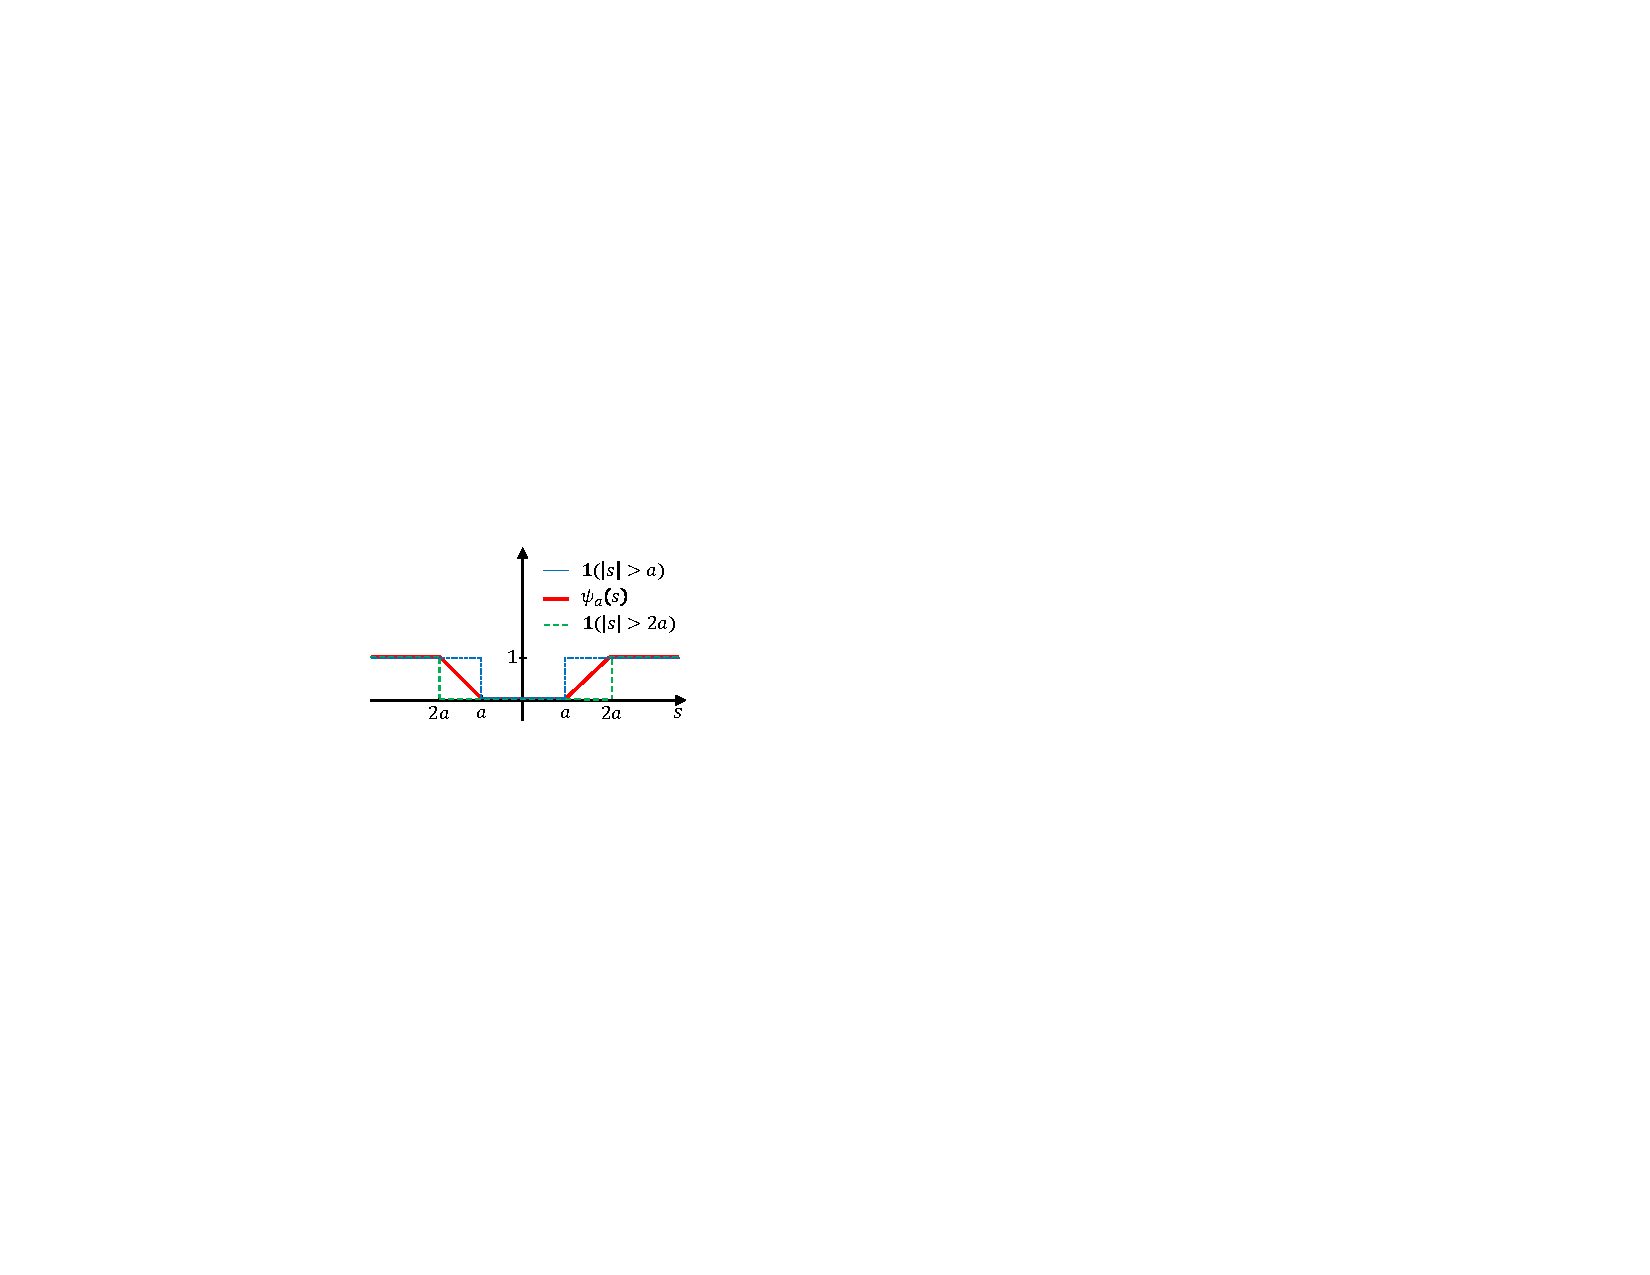
\includegraphics[width=.6\textwidth]{./img/funcs.pdf}				
		\caption{$\indic(|s|> 2a) \leq \psi_a (s) \leq \indic(|s|>a)$}
		\label{funcs}
	\end{figure}

	Now using the definition of the marginal tail function we have:
	\be 	
	\nr 
	\ex \sup_{\ddelta \in \cH} \sum_{g=1}^{G} \xi_g  \sum_{i=1}^{n_g} \left[Q_{2 \xi_g}(\ddelta_{0g})  - \indic (|\langle \x_{gi}, \ddelta_{0g} \rangle| \geq \xi_g )  \right]
	&=& \ex \sup_{\ddelta \in \cH} \sum_{g=1}^{G} \xi_g  \sum_{i=1}^{n_g} \left[\ex \indic (|\langle \x_{gi}, \ddelta_{0g} \rangle| \geq 2\xi_g )   - \indic (|\langle \x_{gi}, \ddelta_{0g} \rangle| \geq \xi_g )  \right] 
	\\ \nr 
	(\text{Figure \ref{funcs}}) &\leq& 
	\ex \sup_{\ddelta \in \cH} \sum_{g=1}^{G} \xi_g  \sum_{i=1}^{n_g} \left[\ex \psi_{\xi_g }(\langle \x, \ddelta_{0g} \rangle)   - \psi_{\xi_g }(\langle \x_{gi}, \ddelta_{0g} \rangle)   \right] 
	\\ \nr  
	(\text{Symmetrization \cite{Vaart1996-zl}}) &\leq& 
	2 \ex \sup_{\ddelta \in \cH} \sum_{g=1}^{G} \xi_g  \sum_{i=1}^{n_g} \epsilon_{gi} \psi_{\xi_g }(\langle \x_{gi}, \ddelta_{0g} \rangle)
	\\ \nr 
	(\text{Rademacher comparison principle \cite{Ledoux1991-ix}}) &\leq& 
	2 \ex \sup_{\ddelta \in \cH} \sum_{g=1}^{G} \sum_{i=1}^{n_g} \epsilon_{gi} \langle \x_{gi}, \ddelta_{0g} \rangle
	\ee  
	where $\epsilon_{gi}$ are iid copies of Rademacher random variable which are independent of every other random variables and themselves.

	Now we add back $\frac{1}{n}$ and expand $\ddelta_{0g} = \ddelta_{0} + \ddelta_{g}$. Also, we substitute $\ddelta \in \cH$ constraint with $\ddelta \in \cC$ because $\cH \subseteq \cC$ where $\cC = \{ \ddelta = (\ddelta_0^T, \dots, \ddelta_G^T)^T \Big| \ddelta_g \in \cC_g \}$. 
	\be 
	\nr 
	\frac{2}{n} \ex \sup_{\ddelta \in \cC} \sum_{g=1}^{G} \sum_{i=1}^{n_g} \epsilon_{gi} \langle \x_{gi}, \ddelta_{0g} \rangle
	&=& \frac{2}{n} \ex \sup_{\ddelta_0 \in \cC_0} \sum_{i=1}^{n} \epsilon_{i} \langle \x_{i}, \ddelta_{0} \rangle
	+ \frac{2}{n} \ex \sup_{\forall g \in [G]: \ddelta_g \in \cC_g} \sum_{g=1}^{G} \sum_{i=1}^{n_g} \epsilon_{gi} \langle \x_{gi}, \ddelta_{g} \rangle
	\\ \nr 
	&=&
	\frac{2}{\sqrt{n}} \ex \sup_{\ddelta_0 \in \cC_0} \sum_{i=1}^{n} \langle \frac{1}{\sqrt{n}} \epsilon_{i} \x_{i}, \ddelta_{0} \rangle
	+ \frac{2}{\sqrt{n}} \ex \sup_{\ddelta_{[G]\setminus} \in \cC_{[G]\setminus}} \sum_{g=1}^{G}  \sqrt{\frac{n_g}{n}} \sum_{i=1}^{n_g} \langle \frac{1}{\sqrt{n_g}} \epsilon_{gi} \x_{gi}, \ddelta_{g} \rangle
	\\ \nr 
	(n_0 := n, \epsilon_{0i} := \epsilon_0, \x_{0i} := \x_i) &=& \frac{2}{\sqrt{n}} \ex \sup_{\forall g \in [G_+]: \ddelta_g \in \cC_g} \sum_{g=0}^{G}  \sqrt{\frac{n_g}{n}} \sum_{i=1}^{n_g} \langle \frac{1}{\sqrt{n_g}} \epsilon_{gi} \x_{gi}, \ddelta_{g} \rangle
	\\ \nr 
	(\h_{g} := \frac{1}{\sqrt{n_g}} \sum_{i=1}^{n_g} \epsilon_{gi} \x_{gi}) &=& \frac{2}{\sqrt{n}} \ex \sup_{\forall g \in [G_+]: \ddelta_g \in \cC_g} \sum_{g=0}^{G}  \sqrt{\frac{n_g}{n}}  \langle \h_{g}, \ddelta_{g} \rangle
	\\ \nr 
	(\u_g \in \ddelta_g/\norm{\ddelta_g}{2}, \cA_g \in \cC_g \cap \sphere) &\leq& \frac{2}{\sqrt{n}} \ex \sup_{\forall g \in [G_+]: \u_g \in \cA_{g}} \sum_{g=0}^{G}  \sqrt{\frac{n_g}{n}} \langle \h_{g}, \u_{g} \rangle \norm{\ddelta_{g}}{2}
	\\ \nr 
	(\sup \sum < \sum \sup) &\leq& \frac{2}{\sqrt{n}} \sum_{g=0}^{G}  \sqrt{\frac{n_g}{n}} \ex_{\h_{g}} \sup_{\u_g \in \cA_g}  \langle \h_{g}, \u_{g} \rangle \norm{\ddelta_{g}}{2}
	\\ \nr 
	&\leq& \frac{2}{\sqrt{n}} \sum_{g=0}^{G}  \sqrt{\frac{n_g}{n}} c_g k_x \omega(\cA_g) \norm{\ddelta_{g}}{2}
	\ee
	Note that the $\h_{gi}$ is a sub-Gaussian random vector which let us bound the $\ex \sup$ using the Gaussian width \cite{trop15} in the last step. 
\end{proof}

\subsection{Proof of Lemma \ref{lemm:mainlem}}
\begin{proof} 
	To avoid cluttering let $h_g(\w_g, \X_g) \triangleq \norm{\w_g}{2} \sup_{\u_g \in \cA_g} \langle \X_g^T \frac{\w_g}{\norm{\w_g}{2}}, \u_g \rangle $ be a random quantity and $e_g(\tau) \triangleq c_g k_x (\omega(\cA_g)+\sqrt{\log (G+1)} + \tau)$, and $s_g \triangleq \sqrt{(2k_w^2 + 1)n_g}$ constants. From the law of total probability, we have:	
	\be
	\nr 
	\pr\left( h_g(\w_g , \X_g) >  s_g e_g(\tau) \right) 
	&=& \pr \left( h_g(\w_g , \X_g) >  s_g e_g(\tau) \Big| \norm{\w_g}{2} > s_g \right) \pr\left(\norm{\w_g}{2} > s_g\right) \\ 
	\nr
	&+& \pr \left( h_g(\w_g , \X_g) >  s_g e_g(\tau) \Big| \norm{\w_g}{2} < s_g \right) \pr\left(\norm{\w_g}{2} < s_g\right) \\ 
	\nr 
	&\leq& \pr\left(\norm{\w_g}{2} > s_g \right) + \pr \left( \norm{\w_g}{2} \sup_{\u_g \in \cA_g} \langle \X_g^T \frac{\w_g}{\norm{\w_g}{2}}, \u_g \rangle >  s_g e_g(\tau) \Big| \norm{\w_g}{2} < s_g \right) \\
	\nr 
	&\leq& \pr\left(\norm{\w_g}{2} > \sqrt{(2k_w^2 + 1)n_g}\right) + \pr \left( \sup_{\u_g \in \cC_g \cap \sphere} \langle \X_g^T \frac{\w_g}{\norm{\w_g}{2}}, \u_g \rangle >  e_g(\tau)  \right) \\
	\label{eq:twoterms} 
	&\leq& \pr\left(\norm{\w_g}{2} > \sqrt{(2k_w^2 + 1)n_g}\right) + \sup_{\v \in \sphere}\pr \left( \sup_{\u_g \in \cC_g \cap \sphere} \langle \X_g^T \v , \u_g \rangle >  e_g(\tau)  \right)
	\ee 
	Let's focus on the first term. 
	Since $\w_g$ consists of i.i.d. centered unit-variance sub-Gaussian elements with $\normth{w_{gi}}{\psi_2} < k_w$, $w_{gi}^2$ is sub-exponential with $\normth{\w_{gi}}{\psi_1} < 2k_w^2$. 
	Let's apply the Bernstein’s inequality \cite{boucheron13} to $\norm{\w_g}{2}^2 = \sum_{i=1}^{n_g} \w_{gi}^2$:
	\be 
	\nr 
	\pr\left( \big| \norm{\w_g}{2}^2  - \ex\norm{\w_g}{2}^2  \big|  > \tau \right) \leq 
	2 \exp\left(-\nu  \min\left[\frac{\tau^2}{4k_w^4n_g}, \frac{\tau }{2k_w^2}\right]\right) 
	\ee
	We also know that $\ex \norm{\w_g}{2}^2 \leq n_g$ \cite{vershynin2018high} which gives us:
	\be
	\nr 
	\pr\left( \norm{\w_g}{2}  > \sqrt{n_g + \tau } \right) \leq 
	2 \exp\left(-\nu  \min\left[\frac{\tau^2}{4k_w^4n_g}, \frac{\tau }{2k_w^2}\right]\right)
	\ee	
	Finally, we set $\tau = 2k_w^2 n_g$:
	\be
	\nr 
	\label{eq:omeggg}
	\pr\left( \norm{\oomega_g}{2}  > \sqrt{(2k_w^2 + 1)n_g } \right) 
	&\leq& 2\exp\left(-\nu n_g \right) = \frac{2}{(G+1)} \exp\left(-\nu n_g + \log (G+1)\right)
	\ee 
%	Finally, we set $\tau = 2k_w^2 (n_g + \frac{\log(G+1)}{\nu_g})$:
%	\be
%	\nr 
%	%\label{eq:omeggg}
%	&&\pr\left( \norm{\oomega_g}{2}  > \sqrt{(2k_w^2 + 1) (n_g + \frac{\log(G+1)}{\nu_g}) } \right) 
%	\leq 2\exp\left(-\nu_g \min\left[\frac{\left(n_g + \frac{\log(G+1)}{\nu_g}\right)^2}{n_g}, \left(n_g + \frac{\log(G+1)}{\nu_g}\right) \right] \right) 
%	\\ \nr
%	&\leq& 2\exp\left(-\nu_g \min\left[(n_g + \frac{2\log(G+1)}{v_g} + \frac{\log^2(G+1)}{\nu_g^2 n_g}), (n_g + \frac{\log(G+1)}{\nu_g}) \right] \right) 
%	\\ \nr
%	&\leq& 2\exp\left(-\nu_g n_g - \log(G+1) \right) 
%	\\ \nr
%	&=& \frac{2}{(G+1)} \exp\left(-\nu_g n_g \right)
%	\ee 

	Now we upper bound the second term of \eqref{eq:twoterms}.
	Given any fixed $\v \in \sphere$, $\X_g \v$ is a sub-Gaussian random vector with $\normth{\X_g^T \v}{\psi_2} \leq C_gk_x$ \cite{banerjee14}. 
	From Theorem 9 of \cite{banerjee14} for any $\v \in \sphere$ we have:
	\be 
	\label{eq:widthbound}
	\pr \left( \sup_{\u_g \in \cA_g} \langle \X_g^T \v , \u_g \rangle >  \upsilon_g C_gk_x \omega(\cA_g) + t  \right)
	\leq \pi_g \exp \left( - \left( \frac{t}{\theta_g C_g k_x \phi_g}\right)^2 \right)
	\ee 	
	where $\phi_g = \sup_{\u_g \in \cA_g} \norm{\u_g}{2}$ and in our problem $\phi_g = 1$. 
	To simplify we take $c_g  = C_g \max(\upsilon_g, \theta_g)$ and then substitute $t = c_g k_x (\tau + \sqrt{\log (G+1)})$:
	\be 
	\nr 
	\pr \left( \sup_{\u_g \in \cA_g} \langle \X_g^T \v , \u_g \rangle >  c_gk_x \left(\omega(\cA_g) + \sqrt{\log (G+1)} + \tau\right) \right)
	&\leq& \pi_g \exp \left( - \left( \tau + \sqrt{\log (G+1)} \right)^2 \right) \\ 
	\nr 
	&\leq& \pi_g \exp \left( - \log (G+1) - \tau^2 \right) \\ 
	\nr 
	&\leq& \frac{\pi_g}{(G+1)} \exp (-\tau^2)
	\ee 	
	Now we put back results to the original inequality \eqref{eq:twoterms}:
	\be 
	\nr
	&& \pr\left( h_g(\w_g , \X_g) >  \sqrt{(2k_w^2 + 1)n_g} \times c_g k_x \left(\omega(\cA_g)+\sqrt{\log (G+1)} + \tau\right) \right) 
	\\ \nr 
	&\leq& \frac{2}{(G+1)} \exp\left(-\nu n_g + \log (G+1)\right) + \frac{\pi_g}{(G+1)} \exp\left(-\tau^2\right) \\ 
	\nr 
	&\leq& \frac{\sigma_g}{(G+1)} \exp\left(-\min\left[\nu  n_g - \log (G+1), \tau^2\right]\right) 
	\ee 
	where $\sigma_g = \pi_g + 2$.
\end{proof}

\subsection{Proof of Lemma \ref{lem:recurse}}
\begin{proof}
	We upper bound the individual error $\norm{\ddelta_g^{(t+1)}}{2}$ and the common one $\norm{\ddelta_0^{(t+1)}}{2}$ in the followings:
	\be
	\nr 
	\norm{\ddelta_g^{(t+1)}}{2} &=& \norm{\bbeta _g^{(t+1)} - \bbeta _g^*}{2} \\ \nr  
	&=& \normlr{\Pi_{\Omega_{f_g}} \bigg(\bbeta_g^{(t)} + \mu_g \X_g^T \Big(\y_g - \X_g \big(\bbeta_0^{(t)} + \bbeta_g^{(t)}\big) \Big) \bigg) - \bbeta _g^*}{2} \\ \nr 
	\text{(Lemma 6.3 of \cite{oyrs15})}&=& \normlr{\Pi_{\Omega_{f_g}-\{ \bbeta _g^* \}} \bigg(\bbeta_g^{(t)} + \mu_g \X_g^T \Big(\y_g - \X_g \big(\bbeta_0^{(t)} + \bbeta_g^{(t)}\big) \Big) - \bbeta _g^* \bigg)}{2} \\ \nr 
	&=& \normlr{\Pi_{\cE_g} \bigg(\ddelta_g^{(t)} + \mu_g \X_g^T \Big(\y_g - \X_g \big(\bbeta_0^{(t)} + \bbeta_g^{(t)}\big) - \X_g \big(\bbeta _0^* + \bbeta _g^* \big) + \X_g \big(\bbeta _0^* + \bbeta _g^*\big) \Big) \bigg)}{2} \\ \nr 
	&=& \normlr{\Pi_{\cE_g} \bigg(\ddelta_g^{(t)} + \mu_g \X_g^T \Big(\oomega_g - \X_g \big(\ddelta_0^{(t)}  + \ddelta_g^{(t)}\big) \Big) \bigg)}{2} \\ \nr 
	\text{(Lemma 6.4 of \cite{oyrs15})}&\leq&  \normlr{\Pi_{\cC_g} \bigg(\ddelta_g^{(t)} + \mu_g \X_g^T \Big(\oomega_g - \X_g \big(\ddelta_0^{(t)}  + \ddelta_g^{(t)}\big) \Big) \bigg)}{2} \\ \nr 
	\text{(Lemma 6.2 of \cite{oyrs15})}&\leq&  \sup_{\v \in \cC_g \cap \ball} \v^T \bigg(\ddelta_g^{(t)} + \mu_g \X_g^T \Big(\oomega_g - \X_g \big(\ddelta_0^{(t)}  + \ddelta_g^{(t)}\big) \Big) \bigg) \\ \nr
	(\cB_g =  \cC_g \cap \ball) &=&  \sup_{\v \in \cB_g} \v^T \bigg(\ddelta_g^{(t)} + \mu_g \X_g^T \Big(\oomega_g - \X_g \big(\ddelta_0^{(t)}  + \ddelta_g^{(t)}\big) \Big) \bigg) \\ \nr
	&\leq&  \sup_{\v \in \cB_g} \v^T \big(\I_g - \mu_g \X_g^T \X_g\big) \ddelta_g^{(t)} +  \mu_g \sup_{\v \in \cB_g} \v^T \X_g^T \oomega_g  +  \mu_g \sup_{\v \in \cB_g} -\v^T \X_g^T \X_g \ddelta_0^{(t)}   \\ \nr
	&\leq&  \normlr{\ddelta_g^{(t)}}{2} \sup_{\u, \v \in \cB_g} \v^T \big(\I_g - \mu_g \X_g^T \X_g\big) \u  +  \mu_g \norm{\oomega_g}{2} \sup_{\v \in \cB_g} \v^T \X_g^T \frac{\oomega_g}{\norm{\oomega_g}{2}}  \\ \nr 
	&+&  \mu_g  \norm{\ddelta_0^{(t)} }{2}  \sup_{\v \in \cB_g, \u \in \cB_0} -\v^T \X_g^T \X_g \u \\ \nr   
	&=&  \rho_g(\mu_g)\norm{\ddelta_g^{(t)}}{2}   +   \xi_g(\mu_g) \norm{\oomega_g}{2} +  \phi_g(\mu_g) \norm{\ddelta_0^{(t)}}{2} 
	\ee 
	%	where $\theta_f = 1$ for convex $f$ and $\theta_f = 2$ for the non-convex case. 
	%	Note that the last term is lower bounded by zero. To see this clearly consider the set $\cB_{0g} = \{\ddelta_0 + \ddelta_{g} | \ddelta_0 \in \cC_0, \ddelta_g \in \cC_g, \norm{\ddelta_0 + \ddelta_g}{2} \leq 1\}$ where $\cB_0, \cB_g \subseteq \cB_{0g}$:
	%	\be 
	%	\label{eq:zerolb}
	%	\inf_{\v \in \cB_g, \u \in \cB_0} \v^T \X_g^T \X_g \u &\geq& \inf_{\u \in \cB_{0g}} \norm{\X_g \u}{2}^2 \geq 0
	%	\ee 
	So the final bound becomes:
	\be 
	\label{eq:optg}
	\norm{\ddelta_g^{(t+1)}}{2} &\leq&   \rho_g(\mu_g)\norm{\ddelta_g^{(t)}}{2}   +  \xi_g(\mu_g) \norm{\oomega_g}{2} + \phi_g(\mu_g) \norm{\ddelta_0^{(t)}}{2} 
	\ee 	
	Now we upper bound the error of common parameter. Remember common parameter's update:
	$\bbeta _0^{(t+1)} = \Pi_{\Omega_{f_0}} \left(\bbeta_0^{(t)} + \mu_0 \X_0^T   
	\begin{pmatrix}
	(\y_1 - \X_1 (\bbeta_0^{(t)} + \bbeta _1^{(t)}))     \\
	\vdots 	 \\
	(\y_G - \X_G (\bbeta_0^{(t)} + \bbeta _G^{(t)})) 
	\end{pmatrix}\right)$.
	\be 
	\nr 
	\norm{\ddelta_0^{(t+1)}}{2} &=& \norm{\bbeta _0^{(t+1)} - \bbeta _0^*}{2} \\ \nr  \\ \nr 
	&=& \normlr{\Pi_{\Omega_{f_0}} \bigg(\bbeta_0^{(t)} + \mu_0 \sum_{g = 1}^{G} \X_g^T \Big(\y_g - \X_g (\bbeta_0^{(t)} + \bbeta_g^{(t)}) \Big) \bigg) - \bbeta _0^*}{2} \\ \nr 
	\text{(Lemma 6.3 of \cite{oyrs15})} &=& \normlr{\Pi_{\Omega_{f_0}-\{ \bbeta _0^* \}} \bigg(\bbeta_0^{(t)} + \mu_0 \sum_{g = 1}^{G}   \X_g^T \Big(\y_g - \X_g (\bbeta_0^{(t)} + \bbeta_g^{(t)}) \Big) - \bbeta _0^* \bigg)}{2} \\ \nr 
	%		&=& \normlr{\Pi_{\cE_0} \bigg(\ddelta_0^{(t)} + \mu_0 \X_0^T \Big(\y - \X_0 \bbeta_0^{(t)} - \tD \bbeta _{1:g}^{t} - \X_0 \bbeta _0^* - \tD \bbeta _{1:g}^* + \X_0 \bbeta _0^* + \tD \bbeta _{1:g}^*   \Big) \bigg)}{2} \\ \nr 
	%		&=& \normlr{\Pi_{\cE_0} \bigg(\ddelta_0^{(t)} + \mu_0 \X_0^T \Big(\oomega - \X_0 \big( \bbeta_0^{(t)} - \bbeta _0^* \big) - \tD \big( \bbeta _{1:g}^{t} - \bbeta _{1:g}^*  \big) \Big) \bigg)}{2} \\ \nr 
	&=& \normlr{\Pi_{\cE_0} \bigg(\ddelta_0^{(t)} + \mu_0\sum_{g = 1}^{G}   \X_g^T \Big(\y_g - \X_g (\bbeta_0^{(t)} + \bbeta_g^{(t)}) \Big)}{2} \\ \nr 
	\text{(Lemma 6.4 of \cite{oyrs15})} &\leq&  \normlr{\Pi_{\cC_0} \bigg(\ddelta_0^{(t)} + \mu_0 \sum_{g = 1}^{G}   \X_g^T \Big(\oomega_g - \X_g (\ddelta_0^{(t)} + \ddelta_g^{(t)}) \Big) \bigg)}{2} \\ \nr 
	\text{(Lemma 6.2 of \cite{oyrs15})} &\leq&   \sup_{\v \in \cB_0 } \v^T \bigg(\ddelta_0^{(t)} + \mu_0 \sum_{g = 1}^{G}   \X_g^T \Big(\oomega_g - \X_g (\ddelta_0^{(t)} + \ddelta_g^{(t)}) \Big) \bigg)%, \quad \cB_0 =  \cC_0 \cap \ball 
	\\ \nr
	&\leq&  \sup_{\v \in \cB_0} \v^T \big(\I - \mu_0 \sum_{g = 1}^{G}   \X_g^T\X_g  \big) \ddelta_0^{(t)} +  \mu_0 \sup_{\v \in \cB_0} \v^T \sum_{g = 1}^{G}   \X_g^T \oomega_g 
	\\ \nr 
	&+&  \mu_0 \sup_{\v \in \cB_0}  -\v^T \sum_{g=1}^{G}   \X_g^T \X_g \ddelta_g^{(t)}
	\\ \nr 
	&\leq&  \norm{\ddelta_0^{(t)}}{2} \sup_{\u, \v \in \cB_0} \v^T \big(\I - \mu_0 \X_0^T\X_0  \big) \u  +  \mu_0 \sup_{\v \in \cB_0} \v^T \X_0^T \frac{\oomega_0}{\norm{\oomega_0}{2}} \norm{\oomega_0}{2} 
	\\ \nr 
	&+&  \mu_0 \sum_{g=1}^{G}  \sup_{\v_g \in \cB_0, \u_g \in \cB_g} - \v_g^T \X_g^T \X_g \u_g \norm{\ddelta_g^{(t)}}{2} \\ \label{rewrite}
	&\leq&  \rho_0(\mu_0) \norm{\ddelta_0^{(t)}}{2}   +  \xi_0(\mu_0) \norm{\oomega_0}{2} +  \mu_0 \sum_{g=1}^{G}  \frac{\phi_g(\mu_g)}{\mu_g} \norm{\ddelta_g^{(t)}}{2} \\ \nr 
	\ee 
	
	To avoid cluttering we drop $\mu_g$ as the arguments.
	Putting together \eqref{eq:optg} and \eqref{rewrite} inequalities we reach to the followings: 
	\be 
	\nr 
	\norm{\ddelta_g^{(t+1)}}{2} &\leq&   \rho_g\norm{\ddelta_g^{(t)}}{2}   +  \xi_g \norm{\oomega_g}{2} + \phi_g \norm{\ddelta_0^{(t)}}{2} 
	\\ \nr 
	\norm{\ddelta_0^{(t+1)}}{2} &\leq& \rho_0 \norm{\ddelta_0^{(t)}}{2} + \xi_0 \norm{\oomega_0}{2} + \mu_0 \sum_{g=1}^{G}  \frac{\phi_g}{\mu_g} \norm{\ddelta_g^{(t)}}{2}  
	\ee 
\end{proof}

\subsection{Proof of Lemma \ref{lemm:hpub}}
We will need the following lemma in our proof. 
It establishes the RE condition for individual isotropic sub-Gaussian designs and provides us with the essential tool for proving high probability bounds.  
\begin{lemma}[Theorem 11 of \cite{banerjee14}]
	\label{lem:gennips}
	%To unify the illustration assume, $n_0 = n$ and $\X_0 = \oomega$.
	For all $g \in [G]$, for the matrix $\X_g \in \reals^{n_g \times p}$ with independent isotropic sub-Gaussian rows, i.e., $\normth{\x_{gi}}{\psi_2} \leq k$ and $\ex[\x_{gi} \x_{gi}^T] = \I$, the following result holds with probability at least $1 - 2\exp\left( -\gamma_g (\omega(\cA_g) + \tau)^2  \right)$ for $\tau > 0$:
	\be 
	\nr 
	\forall \u_g \in \cC_g: n_g \left(1 -  c_g\frac{\omega(\cA_g) + \tau}{\sqrt{n_g}}\right) \norm{\u_g}{2}^2  \leq \norm{\X_g\u_g}{2}^2 \leq n_g \left(1 +  c_g\frac{\omega(\cA_g) + \tau}{\sqrt{n_g}}\right) \norm{\u_g}{2}^2
	\ee 
	where $c_g > 0$ is constant.% and $(x)_+ = \max(x, 0)$. 
\end{lemma} 

The statement of Lemma \ref{lem:gennips} characterizes the distortion in the Euclidean distance between points $\u_g \in \cC_g$ when the matrix $\X_g/n_g$ is applied to them and states that any sub-Gaussian design matrix is approximately isometry, with high probability:
\be 
\nr 
(1 -  \alpha) \norm{\u_g}{2}^2 \leq \frac{1}{n_g}\norm{\X_g\u_g}{2}^2 \leq (1 + \alpha) \norm{\u_g}{2}^2
\ee 
where $\alpha = c_g \frac{\omega(\cA_g)}{\sqrt{n_g}}$.
Now the proof for Lemma \ref{lemm:hpub}: 
\begin{proof}
	First we upper bound each of the coefficients $\forall  g \in [G]$:
	\be 
	\nr 
	\rho_g(\mu_g) &=& \sup_{\u, \v \in \cB_g} \v^T \big(\I_g - \mu_g \X_g^T \X_g\big) \u  \nr 
	\ee
	
	We upper bound the argument of the $\sup$ as follows:	
	\be 
	\nr 
	\v^T \big(\I_g - \mu_g \X_g^T \X_g\big) \u 
	&=& \frac{1}{4}\left[(\u + \v)^T(\I - \mu_g \X_g^T \X_g) (\u + \v) - (\u - \v)^T(\I - \mu_g \X_g^T \X_g) (\u - \v) \right] \\ \nr 
	&=& \frac{1}{4}\left[\norm{\u + \v}{2}^2 - \mu_g \norm{\X_g(\u + \v)}{2}^2 - \norm{\u - \v}{2}^2 + \mu_g \norm{\X_g(\u - \v)}{2}^2 \right] \\ \nr 
	\text{(Lemma \ref{lem:gennips})} &\leq& \frac{1}{4}\Bigg[\left(1 - \mu_g n_g \left(1 -  c_g\frac{2 \omega(\cA_g) + \tau}{\sqrt{n_g}}\right)\right) \norm{\u + \v}{2} \\ \nr 
	&-& \left(1 - \mu_g n_g \left(1 +  c_g\frac{2 \omega(\cA_g) + \tau}{\sqrt{n_g}}\right)\right) \norm{\u - \v}{2} \Bigg]\\ \nr 
	\\ \nr 
	\left(\mu_g = \frac{1}{a_g n_g}\right) &\leq& \frac{1}{4}\Bigg[\left(1 - \frac{1}{a_g} \right) \left(\norm{\u + \v}{2}  - \norm{\u - \v}{2} \right) +   c_g\frac{2 \omega(\cA_g) + \tau}{a_g \sqrt{n_g}} \left(\norm{\u + \v}{2} + \norm{\u - \v}{2} \right) \Bigg]\\ \nr 
	&\leq& \frac{1}{4}\Bigg[\left(1 - \frac{1}{a_g} \right) 2\norm{\v}{2} +   c_g\frac{2 \omega(\cA_g) + \tau}{a_g \sqrt{n_g}} 2\sqrt{2} \Bigg]\\ \nr 
	\ee 
	where the last line follows from the triangle inequality and the fact that $\norm{\u + \v}{2} + \norm{\u - \v}{2} \leq 2\sqrt{2}$ which itself follows from $\norm{\u + \v}{2}^2 + \norm{\u - \v}{2}^2 \leq 4$.
	Note that we applied the Lemma \ref{lem:gennips} for bigger sets of $\cA_g + \cA_g$ and $\cA_g - \cA_g$ where Gaussian width of both of them are upper bounded by $2\omega(\cA_g)$.
	The above holds with high probability (computed below). %at least $1 - 2\exp\left( -\gamma_g (\omega(\cA_g) + \tau)^2  \right)$.
	Now we set :
	\be 
	\label{eq:rhoub}
	\v^T \big(\I_g - \frac{1}{a_g n_g} \X_g^T \X_g\big) \u 
	&\leq& \frac{1}{2}  \left[\left(1 - \frac{1}{a_g} \right) + \sqrt{2} c_g\frac{2 \omega(\cA_g) + \tau}{a_g \sqrt{n_g}} \right]
	\ee 
	
	To keep the upper bound of $\rho_g$ in \eqref{eq:rhoub} below any arbitrary $\frac{1}{b} < 1$  we need $n_g = O(b^2(\omega(\cA_g) + \tau)^2)$ samples.% which completes the proof. 
	
	Now we rewrite the same analysis using the tail bounds for the coefficients to clarify the probabilities. 
	Let's set $\mu_g = \frac{1}{a_g n_g}$, $d_g := \frac{1}{2}\left(1 - \frac{1}{a_g} \right) + \sqrt{2} c_g\frac{\omega(\cA_g) + \tau/2}{a_g \sqrt{n_g}}$ and name the bad events of $\norm{\X_g(\u + \v)}{2}^2 < n_g \left(1 -  c_g\frac{2 \omega(\cA_g) + \tau}{\sqrt{n_g}}\right) $ and $\norm{\X_g(\u - \v)}{2}^2 > n_g \left(1 +  c_g\frac{2 \omega(\cA_g) + \tau}{\sqrt{n_g}}\right)$ as $\cE_1$ and $\cE_2$ respectively:
	\be 
	\nr 
	\pr(\rho_g \geq d_g) 
	&\leq& \pr(\rho_g \geq d_g | \neg\cE_1, \neg\cE_2) + 2 \pr(\cE_1) + \pr(\cE_2)  
	\\ \nr 
	\text{Lemma \ref{lem:gennips}} &\leq& 0 + 6 \exp\left( -\gamma_g (\omega(\cA_g) + \tau)^2  \right)
	\ee
	which concludes the proof. 	
\end{proof}
		 
%\subsection{Proof of Proposition \ref{prop:2}}
%\begin{proof} 
%	A similar analysis to the proof of Lemma \ref{lemm:hpub} shows the following bound with probability at least $1 - 6\exp\left( -\gamma_g (\omega(\cA_g) + \tau)^2  \right)$ :
%	\be 
%	\nr 
%	\rho_g\left(\frac{1}{\alpha n_g}\right) \leq 2 c_g\frac{\omega(\cA_g) + \tau}{\sqrt{n_g}}. 
%	\ee
%	for $\alpha > 1$.
%	Note that the bound is twice the case in which $\alpha = 1$, i.e, Lemma \ref{lemm:hpub}. 
%	Also, Lemma \ref{lemm:mainlem} readily provides a high probability upper bound for $\eta_g(1/(\alpha n_g))$ as $\sqrt{(2K^2 + 1)}/\alpha \left(\zeta_g k \omega(\cA_g) + \epsilon_g \sqrt{\log G} +  \tau \right)/\sqrt{n_g}$.
%	Replacing $\alpha$ with $G+1$ and redoing the proof of Theorem \ref{theo:step} completes the proof. 
%\end{proof}


%\subsection{Proof of Lemma \ref{lemm:simp}}
%	We simply write the law of total probability:
%	\be 
%	\nr 
%	\pr \left(XY \leq ab \right) &=& \pr (XY \leq ab | X \leq a ) \pr(X \leq a) + \pr (XY \leq ab | X > a ) \pr(X > a) 
%	\\ \nr 
%	&\leq& \pr(X \leq a) + \pr (XY \leq ab | X > a )  
%	\\ \nr 
%	&=& \pr(X \leq a) + \int_{-\infty}^{\infty} \int_{a}^{\infty} \pr(X =  x, Y = y) \1 (XY \leq ab) dx dy   
%	\\ \nr
%	&\leq& \pr(X \leq a) + \int_{-\infty}^{b} \int_{a}^{\infty} \pr(X =  x, Y = y) \1 (XY \leq ab) dx dy 
%	\\ \nr 
%	&+& \int_{b}^{\infty} \int_{a}^{\infty} \pr(X =  x, Y = y) \1 (XY \leq ab) dx dy   
%	\\ \nr
%	(X > a, Y > b \Rightarrow \1(XY \leq ab) = 0)&\leq& \pr(X \leq a) + \int_{-\infty}^{b} \int_{a}^{\infty} \pr(X =  x, Y = y) \1 (XY \leq ab) dx dy 
%	\\ \nr 	
%	&\leq& \pr(X \leq a) + \int_{-\infty}^{b} \int_{a}^{\infty} \pr(X =  x, Y = y) dx dy 
%	\\ \nr 	
%	&\leq& \pr(X \leq a) + \int_{-\infty}^{b} \int_{-\infty}^{\infty} \pr(X =  x, Y = y) dx dy 
%	\\ \nr 	
%	&\leq& \pr(X \leq a) + \pr(Y \leq b)  
%	\ee 
%	We repeat the same procedure to get the other inequality:
%	\be 
%	\nr 
%	\pr \left(X+Y \leq a+b \right) &\leq&  \pr(X \leq a) + \pr(X + Y \leq a + b | X > a)
%	\\ \nr 
%	&\leq&  \pr(X \leq a) + \int_{-\infty}^{\infty} \int_{a}^{\infty} \pr(X =  x, Y = y) \1 (X+Y \leq a+b) dx dy 
%	\\ \nr 
%	&\leq&  \pr(X \leq a) + \int_{-\infty}^{b} \int_{a}^{\infty} \pr(X =  x, Y = y)  dx dy 
%	\\ \nr 
%	&\leq& \pr(X \leq a) + \pr(Y \leq b)  
%	\ee \qed


\subsection{Proof of Lemma \ref{lemm:phi}}
\begin{proof}
	The following holds for any $\u$ and $\v$ because of $\norm{\X_g (\u + \v)}{2}^2 \geq 0$:
	\be 
	-\v^T \X_g^T \X_g \u \leq \frac{1}{2} \left(\norm{\X_g \u}{2}^2 + \norm{\X_g \v}{2}^2 \right)
	\ee 
	Now we can bound $\phi_g$ as follows:
	\be 
	\phi_g(\mu_g) = \mu_g \sup_{\v \in \cB_g, \u \in \cB_0} -\v^T \X_g^T \X_g \u 
	&\leq& \frac{\mu_g}{2} \left(\sup_{\u \in \cB_0} \norm{\X_g \u}{2}^2 + \sup_{\v \in \cB_g} \norm{\X_g \v}{2}^2 \right)
	\ee 
	So we have:
	\be 
	\phi_g\left(\frac{1}{a_g n_g}\right) 
	&\leq& \frac{1}{2a_g} \left(\frac{1}{n_g}\sup_{\u \in \cB_0} \norm{\X_g \u}{2}^2 + \frac{1}{n_g}\sup_{\v \in \cB_g} \norm{\X_g \v}{2}^2 \right) 
	\\ \nr 
	\text{(Lemma \ref{lem:gennips})} &\leq& \frac{1}{a_g}  \left(1 + c_{0g}\frac{\omega(\cA_g) + \omega(\cA_0) + 2 \tau}{2\sqrt{n_g}} \right)
	\\ \nr 
	(\omega_{0g} = \max(\omega(\cA_0), \omega(\cA_g)) &\leq& \frac{1}{a_g}  \left(1 + c_{0g}\frac{\omega_{0g} + \tau}{\sqrt{n_g}} \right)
	\ee
	where $c_{0g} = \max(c_0, c_g)$. 
	
	To compute the exact probabilities lets define $s_g := \frac{1}{a_g}  \left(1 + c_{0g}\frac{\omega(\cA_g) + \omega(\cA_0) + 2\tau}{2\sqrt{n_g}} \right)$ and name the bad events of $\frac{1}{n_g}\sup_{\u \in \cB_0} \norm{\X_g \u}{2}^2 > 1 + c_{0}\frac{\omega(\cA_0) + \tau}{\sqrt{n_g}}$ and $\frac{1}{n_g}\sup_{\v \in \cB_g} \norm{\X_g \v}{2}^2 > 1 + c_{g}\frac{\omega(\cA_g) + \tau}{\sqrt{n_g}}$ as $\cE_1$ and $\cE_2$ respectively. 
	\be 
	\pr (\phi_g > s_g) 
	&\leq& \pr (\phi_g > s_g | \neg \cE_1) \pr(\neg \cE_1) + \pr(\cE_1)
	\\ \nr
	&\leq& \pr(\cE_2) + \pr(\cE_1)
	\\ \nr
	&\leq& 4\exp\left( -\gamma_g (\omega(\cA_g) + \tau)^2 \right)
	\ee 
\end{proof}


\subsection{Proof of Lemma \ref{paley}}
\begin{proof}
	To obtain lower bound, we use the Paley--Zygmund inequality for the zero-mean, non-degenerate ($0 < \alpha \leq \ex |\langle \x, \u \rangle|, \u \in \sphere$) sub-Gaussian random vector $\x$ with $\normth{\x}{\psi_2} \leq k_x$ \cite{trop15}. 
	\be 
	\nr 
	Q_{2\xi}(\u)  \geq \frac{(\alpha - 2\xi)^2}{4ck_x^2}.
	\ee 	
\end{proof}	

\subsection{Proof of Lemma \ref{incolem main}}
\begin{proof}
	We split $[G]-\cI$ into two groups $\cJ,\cK$. $\cJ$ consists of $\ddelta_g$'s with $\norm{\ddelta_g}{2}\geq 2\norm{\ddelta_0}{2}$ and $\cK=[G]-\cI-\cJ$. We use the bounds
	\[
	\norm{\ddelta_0+\ddelta_g}{2}\geq 
	\begin{cases}
		\lamin(\norm{\ddelta_g}{2}+\norm{\ddelta_0}{2}) &\text{if}~g\in \cI
		\\ 
		\norm{\ddelta_g}{2}/2 &\text{if}~g\in \cJ
		\\
		0 &\text{if}~g\in \cK			
	\end{cases}
	\] 
	This implies
	\[
	\sum_{g=1}^G n_g\norm{\ddelta_0+\ddelta_g}{2}\geq \sum_{g\in \cJ}\frac{n_g}{2}\norm{\ddelta_g}{2}+\lamin\sum_{g\in \cI} n_g (\norm{\ddelta_g}{2}+\norm{\ddelta_0}{2}).
	\]
	Let $S_\cS=\sum_{g\in \cS}n_g\norm{\ddelta_g}{2}$ for $\cS=\cI,\cJ,\cK$.
	We know that over $\cK$, $\norm{\ddelta_g}{2}\leq 2\norm{\ddelta_0}{2}$ which implies $S_\cK = \sum_{g\in \cK}n_g\norm{\ddelta_g}{2}\leq 2\sum_{g\in \cK}n_g\norm{\ddelta_0}{2}\leq 2n\norm{\ddelta_0}{2}$. Set $\rinc=\min\{1/2,\lamin\ratio/3\}$. %=\lamin\ratio/3$.  
	Using $1/2\geq \rinc$, we write:
	\be 
	\nr 
	\sum_{g=1}^G n_g\norm{\ddelta_0+\ddelta_g}{2}
	&\geq& \rinc S_\cJ +\lamin\sum_{g\in \cI}n_g (\norm{\ddelta_g}{2}+\norm{\ddelta_0}{2})
	\\ \nr 
	(S_\cK \leq 2n\norm{\ddelta_0}{2}) &\geq& \rinc S_\cJ +\rinc S_\cK - 2\rinc n\norm{\ddelta_0}{2}+\left(\sum_{g\in \cI} n_g\right)\lamin \norm{\ddelta_0}{2}+\lamin S_{\Ic}
	\\ \nr 
	(\lamin\geq \rinc) &\geq& \rinc (S_\cI + S_\cJ + S_\cK)+ \left(\left(\sum_{g\in \cI} n_g\right)\lamin-2\rinc n\right)\norm{\ddelta_0}{2}.
	\ee 
	Now, observe that, assumption of the Definition \ref{incodef}, $\sum_{g\in \cI} n_g \geq \ratio n$ implies:
	\be 
	\nr 
	\left(\sum_{g\in \cI} n_g\right)\lamin-2\rinc n\geq (\ratio\lamin -2\rinc)n\geq \rinc n.
	\ee 
	Combining all, we obtain:
	\be 
	\nr 
	\sum_{g=1}^Gn_g \norm{\ddelta_0+\ddelta_g}{2} \geq \rinc (S_\cI + S_\cJ + S_\cK + \norm{\ddelta_0}{2}) = \rinc(n\norm{\ddelta_0}{2} +\sum_{g=1}^G n_g\norm{\ddelta_g}{2}).
	\ee 
\end{proof}